%% We use `subfiles' package
\documentclass[preamble.tex]{subfiles}
\begin{document}

\clearpage

\chapter{Array Fusion}
\label{ch:Fusion}

Suppose we have the following computation to perform:

\begin{hscode}
sum (zipWith (*) xs ys)
\end{hscode}

A person familiar with the fundamentals of functional programming is likely to spot the computation of the dot product of two vectors in this snippet of \Haskell code. Indeed, the @zipWith@ list combinator\icomb will element-wise multiply the two vectors @xs@ and @ys@. Quite expectedly the @sum@ combinator will sum the elements of the resulting vector into a scalar value yielding the dot product of @xs@ and @ys@.

This one-liner was an attempt to develop the motivation for the high-level view on numeric computations. It may seem reasonable to replace the lists with arrays and reimplement the same high-level interface in terms of traditional arrays to avoid random memory access penalties as in the case of lists.

Providing an instantly familiar interface without compromising performance has been one of the goals of the \name{Data Parallel Haskell (DPH)}\idph project \cite{PLKC08,CLP+07}. The work described in this essay has been carried out in the context of this project. It will be discussed in more detail in section \ref{sec:DPH}.

However, even if we replaced the lists with arrays and gave efficient implementations to @sum@ and @zipWith@, the resulting algorithm is still likely to be slower than one written by hand in a language such as \C. The @zipWith@ combinator \*produces* an \*intermediate array*\iintermediate containing the element-wise product of the two input vectors. It is immediately \*consumed* by @sum@, yielding the final (scalar) value. Thus the algorithm performs two traversals and allocates another array of the size of the input arrays.

To illustrate the benefit of Array Fusion let us turn to the implementation of same algorithm expressed in \C:


\begin{ccode}
double dotProduct (double xs[], double ys[], int len) {
	// zipWith
	double* temp = malloc(len * sizeof(double));
	for(int i = 0; i < len; i++)
		temp[i] = xs[i] * ys[i];

	// sum
	double result = 0;
	for(int i = 0; i < len; i++)
		result += temp[i];

	return result;
}
\end{ccode}


We immediately notice that both loops iterate over the same \*range* of indices and we could hence perform it as one loop. The two loops are said to have the same \*rate*\irate (the term used more recently in the context of loop fusion in \Haskell \cite{BenLippmeier:2014jc}).


\begin{ccode}
double* temp = malloc(len * sizeof(double));
double result = 0;
for(i = 0; i < len; i++) {
	temp[i] = xs[i] * ys[i];
	result += temp[i];
}
\end{ccode}


\begin{bluebox}
The process of finding and exploiting the opportunities for merging multiple loops into one is referred to as \term{loop fusion}.\ifusion
\end{bluebox}


However, this does not completely bypass the allocation of an intermediate array.\iintermediate Clearly, the intermediate array is redundant and the intermediate value @temp@ could just be a \*scalar* as in the following:


\begin{ccode}
double temp; // temp has become scalar
double result = 0;
for(int i = 0; i < len; i++) {
	temp = xs[i] * ys[i];
	result += temp;
}
\end{ccode}


\begin{bluebox}
The optimisation that removes the need for temporary arrays by replacing them with scalars is called \term{scalarisation}.\idx{scalarisation}
\end{bluebox}


It is a special case of \term{array contraction}.\idx{array contraction} Array contraction optimisation attempts to remove a \*dimension* from the array. In this particular case we contracted a one dimensional array to a scalar, hence \*scalarisation*. However, in the examples with arrays of higher dimensions the dimension could just be reduced, and not eliminated entirely. We will see examples of that in the upcoming chapters when we discuss \*segmented array combinators*.\isegcomb This concept is taken even further in multi-dimensional array systems such as \name{Repa} \cite{KCL+10} and \name{Accelerate} \cite{CKL+11}.


\begin{bluebox}
\term{Loop Fusion} and \term{Array Contraction} optimisation are collectively referred to as \term{Array Fusion}.
\end{bluebox}


Another term for this commonly encountered in literature is \term{deforestation},\idx{deforestation} first coined by Philip Wadler in \cite{Wad90}.

In the remainder of this chapter I identify several types of fusion as well as the shortcomings of the previously available fusion systems which motivated the search for a fresh approach.


%\clearpage
%\section{Types of collective array operations}
%\label{sec:combinator-types}

%In this section I present a classification of collective array operations\icollop that were of primary importance for this project. The classification is based on how the combinators consume\icomb their inputs and produce outputs.

%It is by no means the only way to classify the combinators. However, the analysis is aimed to showcase the different ways in which array combinators may interact with each other is a user program.

%While the discussion of the context of the work and the justification of the choice of combinators is left until the next chapter, we will attempt to put the currently available fusion systems in perspective and determine the combinators and programs for which they perform less effectively.

\clearpage
\section{Types of collective array operations}


\subsection{Simple pipeline fusion}
\label{sec:straight-line}

The most basic form of optimisation that is attempted by most fusion systems is @map/map@ fusion where a pipeline of @map@ combinators is transformed into a single @map@:

\begin{hscode}[mathescape]
map g $\circ$ map f $\mapsto$ map (g $\circ$ f)
\end{hscode}

However, @map@ is not the only combinator that can be chained together in a pipeline. @scan@ and @filter@, like @map@, both \*consume* one array and \*produce* another.
% are both \term{array transducers}\idx{transducer}, in that they \*consume* one array and \*produce* another.

In the simplest case, at the beginning of such a combinator pipeline there is a physical, or \term{manifest}\imanifest array, materialised in memory. However, there may also be a \term{pure producer} or a \term{generator}\igencomb instead. As such @replicate@, @enumerate@ and several others, generate an array from scalars or functions according to some rule.

Just like a pipeline does not necessarily start with a physical array, it may be concluded with a computation such as @fold@ yielding one scalar value.

The combinators discussed so far can be combined into a pipeline of operations where an array output of one combinator is fed directly as input to the next. Additionally, each combinator in the pipeline is able to consume the elements one by one at the \*rate* they are produced by the preceding combinator.

%Assuming that a computation is expressed a pipeline of combinators uninterrupted by \*branching* or \*control flow* are generally handled well by many existing fusion frameworks.

Such simple pipelines are generally handled well by most fusion frameworks. In particular the expressions presented in Figure~\ref{fig:simple-piplines} are all fusible by \name{Stream Fusion} \cite{CLS07} (and Appendix~\ref{sec:stream-fusion}) and \name{Functional Array Fusion} \cite{CK01}.

\begin{figure}
\begin{hscode}
let ys = map (/100)     let s = fold (+) 0       let ws = filter odd
       $ filter (>0)          $ map (^2)                $ map (+1)
       $ xs                   $ scan (*) 1              $ enumFromTo 1 10
                              $ zs
\end{hscode}

\begin{subfigure}{.33\textwidth}%
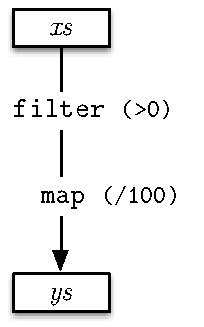
\includegraphics[center]{img/simple-pipeline-a}%
\end{subfigure}%
\begin{subfigure}{.33\textwidth}%
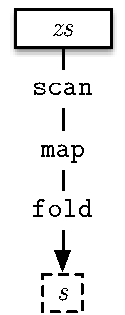
\includegraphics[center]{img/simple-pipeline-b}%
\end{subfigure}%
\begin{subfigure}{.33\textwidth}%
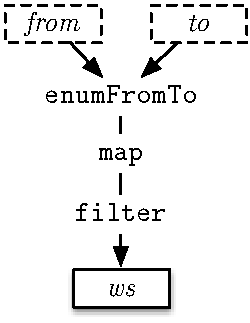
\includegraphics[center]{img/simple-pipeline-c}%
\end{subfigure}%

\caption{Examples of simple combinator pipelines: \Haskell expressions (top) and their corresponding data flow graphs (bottom).}
\label{fig:simple-piplines}
\end{figure}



\subsection{Multi-array consumers fusion}
\label{sec:multiarray-fusion}

A more elaborate and more complex form of fusion involves combinators which accept more that one array as input.


\subsubsection{Point-wise consumers}

The term \term{point-wise} will be used to describe the manner of array processing where multiple arrays are consumed in lockstep.

The most obvious of them is @zipWith@ (and its \codemath{zipWith$N$} counterparts) which has already been used for point-wise multiplication of two vectors in the beginning of this chapter \todo{(also on Figure~\ref{})}:

%\begin{hscode}
%let s = sum
%      $ zipWith (*) xs ys
%\end{hscode}

Another example is a combinator called \*segmented replicate* which given an array of elements and an array of counts creates a new array where each element is repeated the number of times specified by the count, e.g.:

\begin{hscode}
replicate_s [2,1,3] [10,20,30] = [10,10,20,30,30,30]
\end{hscode}


However, point-wise consumption is not the only useful way to consume arrays. Other recurring patterns of consumption of multiple arrays include \term{interleaved}, \term{random access}, \term{consecutive} and \term{nested} which we discuss next.


\subsubsection{Interleaved consumers}

Interleaved consumption presumes picking elements from one array at a time but potentially changing the array to pick from from iteration to iteration. \*Interleave* and \*segmented append* are examples of these. Expectedly interleave picks one element from each array in order, while \*segmented append* interleaves the whole segments of arrays:

\begin{hscode}
interleave [1,3,5,7,9] [2,4,6] = [1,2,3,4,5,6,7,9]

append_s ([2,1,1],[10,20, 30, 40]) ([1,2,2],[50, 60,70, 80,90])
  = [10,20, 50, 30, 60,70, 40, 80,90]
\end{hscode}


\subsubsection{Random access consumers}

Random access pattern is useful for combinators performing \*backwards permutation* on an array given an array of indexes (@bpermute@. In @bpermute@ the indexes specify which elements must be picked from the source array and that array must be randomly accessible:

\begin{hscode}
bpermute [0,10,20,30,40,50] [3,4,5,1] = [30,40,50,10]
\end{hscode}

This is different from \*forward permutation*, where the index array specifies the \*destination* index for a particular index of the source array. This allow one to consume both arrays in a lockstep, where each array is potentially a result of a fused pipeline of operations. However, @permute@ will likely be unable to fuse into its consumer because of out-of-order output generation.

\begin{hscode}
permute [30,40,50,10,20,0] [3,4,5,1,2,0] = [0,10,20,30,40,50]
\end{hscode}


\subsubsection{Consecutive consumers}

This type of consumers is a result of two or more independent array traversals, with one happening after the other. @append@ is currently the only combinator which possesses this property:

\begin{hscode}
append [1,2,3,4,5] [6,7,8] = [1,2,3,4,5, 6,7,8]
\end{hscode}


\subsubsection{Nested consumers}

We have already mentioned a \*segmented replicate* and a \*segmented append* in this section. These types of combinator form the basis of how \DPH handles operations on \*nested* arrays by way of \name{Flattening transform} (Section~\ref{sec:Flattening}). All nested arrays in the \DPH backend are represented by flat data array and a \*segment descriptor* defining the original nesting.

Conceptually \*segmented combinators* resemble nested loops in procedural languages, where for each element taken from the segment descriptor array, that many elements of the data array get processed. We can identify two types of such segmented combinators:
\begin{enumerate}
\item Combinators that \*produce* elements at the \*rate* of the segment descriptor, i.e. one element per segment. For example:

\begin{hscode}
fold_s [3,1,2] max minBound [1,4,2, 5, 6,8] = [4,5,8]
\end{hscode}

\item Combinators that \*produce* elements at the \*rate* of the data array. For example:

\begin{hscode}
scan_s [3,1,2] (+) 0 [1,4,2, 5, 6,8] = [0,1,5, 0, 0,6]
\end{hscode}
\end{enumerate}

As seen in the above examples @fold_s@ and @scan_s@ behave identical to their \name{Prelude} counterparts as applied to individual segments.

There is also a type of segmented combinators which are a segmented equivalent of \*generators*.\igencomb They produce segmented arrays given certain input arrays. These combinators roughly fit in the second category (data rate) even though they don't consume a data array as such. \*Segmented replicate*, \*enumerators* and \*index generator* are all examples of these:

\begin{hscode}
replicate_s [2,1,3] [10,20,30] = [10,10,20,30,30,30]

enumFromStepLenEach [10,40,60] [1,2,3] [2,4,3]
  = [10,11, 40,42,44,46, 60,63,66]

indices_s [5,3,4] = [0,1,2,3,4, 0,1,2, 0,1,2,3]
\end{hscode}


\clearpage
\section{Problems with equational fusion systems}

\subsection{No fusion into multiple consumers}

\subsection{Duplicated loop counters}

\clearpage
\section{An alternative}

In following chapter I will introduce the reader to the \DPH project.
\IfNotCompilingAll{\bibliography{bib}}


\end{document}